% ******************************************************** %
%              TEMPLATE DE INFORME ORGA2 v0.1              %
% ******************************************************** %
% ******************************************************** %
%                                                          %
% ALGUNOS PAQUETES REQUERIDOS (EN UBUNTU):                 %
% ========================================
%                                                          %
% texlive-latex-base                                       %
% texlive-latex-recommended                                %
% texlive-fonts-recommended                                %
% texlive-latex-extra?                                     %
% texlive-lang-spanish (en ubuntu 13.10)                   %
% ******************************************************** %


\documentclass[a4paper]{article}
\usepackage[spanish]{babel}
\usepackage[utf8]{inputenc}
\usepackage{charter}   % tipografia
\usepackage{graphicx}
%\usepackage{makeidx}
\usepackage{paralist} %itemize inline
\usepackage{subcaption}


%\usepackage{float}
%\usepackage{amsmath, amsthm, amssymb}
%\usepackage{amsfonts}
%\usepackage{sectsty}
%\usepackage{charter}
%\usepackage{wrapfig}
%\usepackage{listings}
%\lstset{language=C}

% \setcounter{secnumdepth}{2}
\usepackage{underscore}
\usepackage{caratula}
\usepackage{url}
\usepackage{ragged2e}
\usepackage{hyperref}
\usepackage{pdfpages}


% ********************************************************* %
% ~~~~~~~~              Code snippets             ~~~~~~~~~ %
% ********************************************************* %

\usepackage{color} % para snipets de codigo coloreados
\usepackage{fancybox}  % para el sbox de los snipets de codigo

\definecolor{litegrey}{gray}{0.94}

\newenvironment{codesnippet}{%
	\begin{Sbox}\begin{minipage}{\textwidth}\sffamily\small}%
	{\end{minipage}\end{Sbox}%
		\begin{center}%
		\vspace{-0.4cm}\colorbox{litegrey}{\TheSbox}\end{center}\vspace{0.3cm}}



% ********************************************************* %
% ~~~~~~~~         Formato de las páginas         ~~~~~~~~~ %
% ********************************************************* %

\usepackage{fancyhdr}
\pagestyle{fancy}

%\renewcommand{\chaptermark}[1]{\markboth{#1}{}}
\renewcommand{\sectionmark}[1]{\markright{\thesection\ - #1}}

\fancyhf{}

\fancyhead[LO]{Sección \rightmark} % \thesection\ 
\fancyfoot[LO]{\small{Ivo Pajor, Laureano Muñiz, Luciana Gorosito}}
\fancyfoot[RO]{\thepage}
\renewcommand{\headrulewidth}{0.5pt}
\renewcommand{\footrulewidth}{0.5pt}
\setlength{\hoffset}{-0.8in}
\setlength{\textwidth}{16cm}
%\setlength{\hoffset}{-1.1cm}
%\setlength{\textwidth}{16cm}
\setlength{\headsep}{0.5cm}
\setlength{\textheight}{25cm}
\setlength{\voffset}{-0.7in}
\setlength{\headwidth}{\textwidth}
\setlength{\headheight}{13.1pt}

\renewcommand{\baselinestretch}{1.1}  % line spacing

% ******************************************************** %


\begin{document}


\thispagestyle{empty}
\materia{Organización del Computador II}
\submateria{Segundo Cuatrimestre de 2020}
\titulo{Trabajo Práctico III}
\subtitulo{System Programming}
\integrante{Ivo Pajor}{460/19}{ivo_pajor@hotmail.com}
\integrante{Laureano Muñiz}{498/19}{lau2000m@hotmail.com}
\integrante{Luciana Gorosito}{577/18}{lugorosito0@gmail.com}

\maketitle


\thispagestyle{empty}
\vfill


\thispagestyle{empty}
\vspace{3cm}
\tableofcontents
\newpage


%\normalsize
\newpage

\section{Introducción}
\justify
El objetivo de este trabajo práctico es aplicar gradualmente los conceptos de \textit{System Programming} vistos en las clases teóricas y prácticas, mediante la implementación de una serie de ejercicios que, inspirados en la serie \textit{Rick y Morty}, en conjunto conformarán un kernel o un pequeño sistema operativo. 



\section{Desarrrollo}
\justify
A continuación detallamos las implementaciones de los ejercicios del trabajo práctico.

\subsection{Ejercicio 1}
\justify
Para la realización de este ejercicio analizamos las estructuras \textbf{gdt_entry_t} y \textbf{gdt_descriptor_t} definidas por la cátedra. En esta implementación, la Tabla de Descriptores Globales(GDT) es un arreglo de  \textbf{gdt_entry_t} y su descriptor, que luego cargaremos en GDTR, es del tipo \textbf{gdt_descriptor_t}.\par
\justify
Siguiendo lo indicado en el primer item, definimos a partir del índice 10, 4 descriptores de segmento en la GDT utilizando la estructura \textbf{gdt_entry_t}, atendiendo a las propiedades particulares de cada segmento. Así definimos las entradas de dos segmentos de código de nivel
0 y 3 y de dos segmentos de datos, también de nivel 0 y 3. Puesto que estos segmentos deben direccionar los primeros 201 MB de memoria establecimos en todos el bit de G en 1, y definimos su base en 0x00000000 y su limite en 0x00C8FF. Además, como son segmentos de código o datos de 32 bits, los bit S y D/B se encuentran seteados en 1 y el bit L en 0. Los bits de DPL de cada uno están seteados en 0 o en 3 de acuerdo con el nivel de privilegio que le corresponda. Por último, los bits de tipo están seteados como 0xA en caso de tratarse de un segmento de código y como 0x2 en caso de tratarse de un segmento de datos. En todos, el bit P se setea en 1 para reflejar que los segmentos están presentes. En el caso del bit de AVL, como es un bit reservado lo seteamos en 0.

\begin{figure}[h]
	\centering
	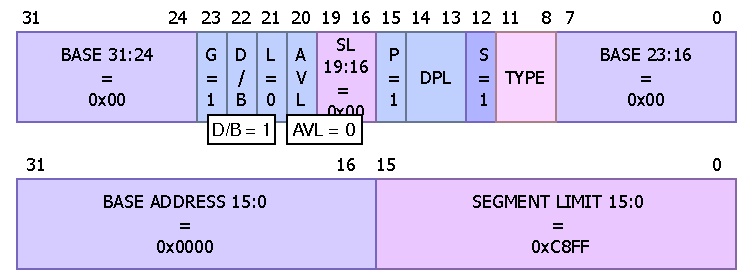
\includegraphics[scale=0.8]{img/GDTdescriptor.pdf}
	\caption{Esquema general de un descriptor de la GDT para los 4 segmentos.}
\end{figure}


\justify
Realizando lo pedido en el item b, pasamos a modo protegido. Para poder hacer esto modificamos el archivo kernel.asm, allí deshablitamos las interrupciones, cargamos en el registro GDTR la estructura \textbf{gdt_descriptor_t} y modificamos el ultimo bit del registro de control CR0, es decir, seteamos en 1 el bit de \textit{Protection Enable}. Posteriormente, escribimos el código necesario para saltar efectivamente a modo protegido. Debido a que este salto se consigue haciendo un \textit{far jump} a la próxima instrucción, designamos una etiqueta llamada \textbf{modo_protegido} a partir de la cual obtendremos el offset, mientras que como selector utilizamos el correspondiente al segmento de código de nivel 0. Además, seteamos la pila del kernel en la dirección 0x25000, es decir, en la base de la pila. Una vez que pasamos a modo protegido, cargamos correctamente los selectores de segmento, en los registros ds, es, fs, gs, ss, usando como registro auxiliar ax, donde se encontraba el selector de segmento de nivel 0 (RPL = 0).


\justify
Seguidamente, definimos otra entrada en la GDT destinada a un segmento de vídeo de nivel 0 (DPL = 0). A diferencia de los cuatro segmentos anteriores, la base de este segmento es distinta de 0, por lo que los campos de la base fueron ser completados con el valor 0x000B8000. Como la pantalla es de 80x50 y como cada pixel ocupa 2 bytes, el límite de este segmento es 0x01F3F. Como este límite entra en 20 bits, el bit de granularidad de este descriptor queda en 0. Además, al ser un segmento de datos de lectura y escritura el tipo es 0x02 y el bit de s queda seteado en 1. Como en las entradas anteriores, los bits de AVL y L quedan en 0, mientras que los bits de present y D/B quedan en 1.  

\begin{figure}[h]
	\centering
	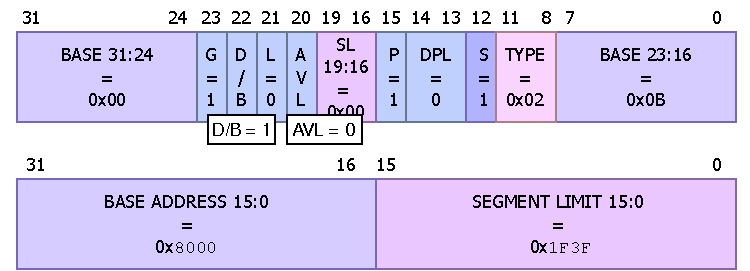
\includegraphics[scale=0.8]{img/DescriptorVideo.pdf}
	\caption{Esquema del descriptor de segmento de video.}
\end{figure}

\justify
Para finalizar este ejercicio, realizamos un rutina encargada de limpiar la pantalla, y pintar el área del mapa de color verde, junto con las barras de los jugadores Rick y Morty. Inicialmente, esta rutina fue implementada en ASM dentro del archivo \textit{kernel.asm}, para corroborar el correcto funcionamiento del acceso al segmento de vídeo, pero luego fue reemplazada por la función en C  "inicializar_pantalla" que se encuentra en el archivo \textit{screen.c}. La pantalla se ve de la siguiente manera:

\begin{figure}[h]
	\centering
	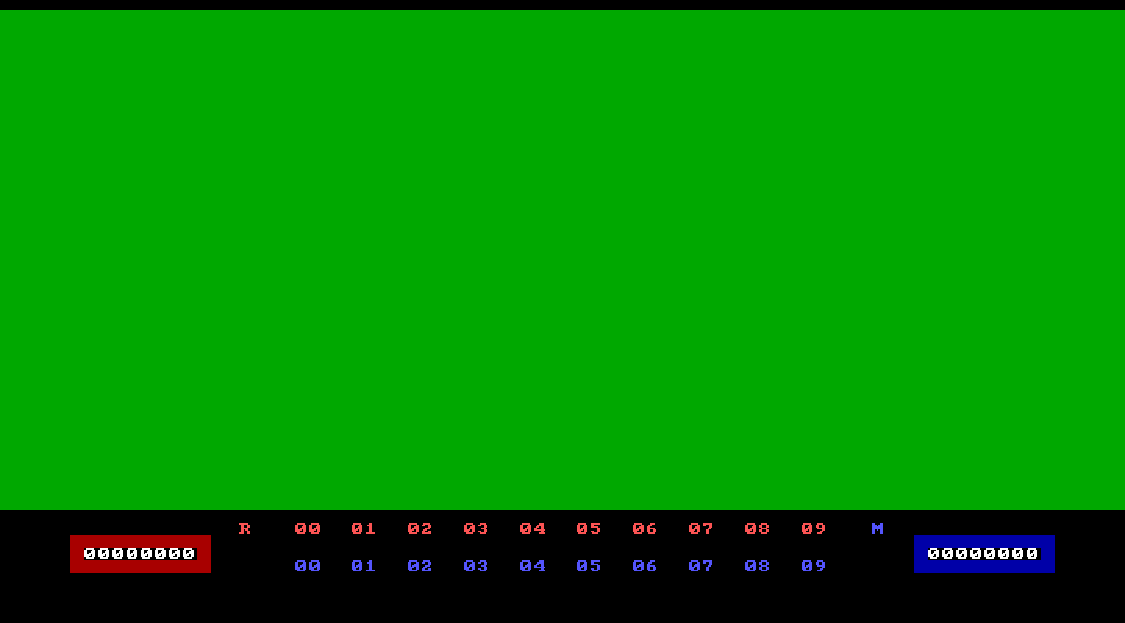
\includegraphics[scale=0.6]{img/Pantalla.pdf}
	\caption{Pantalla inicial.}
\end{figure}


\subsection{Ejercicio 2}
\justify
Inicialmente modificamos los archivos \textit{idt.c} e \textit{idt.h} para completar las entradas de la IDT. Definimos a la IDT como un arreglo de idt_entry_t de 255 posiciones, que primero inicializamos en cero, y el descriptor de la IDT (IDT_DESC), indicando el tamaño y la dirección de la IDT. Para inicializar las entradas de la IDT utilizamos un \textit{DEFINE} que, dado el número de la interrupción, completa los campos del descriptor de la IDT correspondiente. Para el caso de las interrupciones de software el DPL es 3, dado que las mismas deben poder ser accedidas por las tareas y en los demás casos el DPL es 0, ya que no deben poder ser accedidas por las tareas. En todos los casos el selector de segmento es de código de nivel 0, porque las rutinas no pueden ser modificadas por las tareas. Como la dirección de la IDT no está definida en tiempos de compilación fue necesario definir una función llamada idt_init que inicializara las entradas de la IDT en tiempos de ejecución. Definimos 21 entradas en la IDT para las excepciones del procesador(de 0 a 20).
\justify
Para imprimir las excepciones en la esquina superior izquierda de la pantalla  cuando estas ocurren, implementamos la función "print_exception", que se encuentra en el archivo \textit{screen.c}. La misma es llamada inicialmente en el código de \textit{isr.asm}, aunque luego esto será modificado como se ve en el código, ya que esta acción será realizada por el modo debug. 


%Acá va una imagen de un descriptor de la IDT.


\subsection{Ejercicio 3}
\justify
En este ejercicio definimos dos entradas en la IDT para las interrupciones externas o de hardware (32 del clock y 33 del keyboard) y cuatro entradas para las interrupciones de software(88, 89, 100, 123).
\justify
De acuerdo a lo pedido en el segundo, tercer y cuarto item, dentro del archivo \textit{isr.asm} escribimos el esqueleto de las rutinas de interrupciones del reloj, de teclado y de software, que luego irán siendo modificadas a lo largo del transcurso de los ejercicios.

\justify
\textbf{Rutina de interrupción del reloj}
\justify
Esta rutina comienza con un call a la función pic_finish1, para avisar que la interrupción fue atendida. Seguidamente se llama a la función "next_clock", provista por la cátedra. La misma se encarga de imprimir por pantalla una animación del un cursor rotando en la esquina inferior derecha de la pantalla.

\justify
\textbf{Rutina de interrupción del teclado}
\justify
Esta rutina comienza levantando del puerto 0x60 la tecla que fue presionada durante la interrupción. Para que esta tecla sea impresa por pantalla se implementó la función "print_digito" \ en el archivo \textit{screen.c}. Para finalizar, hacemos un call a pic_finish1, para avisar que la interrupción fue atendida.

\justify
\textbf{Rutinas de interrupciones de software}
\justify
Las rutinas de interrupciones de software solo mueven a eax los números indicados por el item d, esto luego será modificado.

\subsection{Ejercicio 4}
\justify
Para inicializar el directorio y las tablas de páginas del kernel, implementamos la función ``mmu_init_kernel_dir", que crea un directorio y una tabla de páginas (tabla_0) del tipo \textit{page_directory_entry}  y \textit{page_table_entry}, respectivamente. Estas estructuras fueron definidas en el archivo \textit{mmu.h} y siguen el formato de las entradas al directorio y a la tabla de páginas. Una vez creados los inicializamos en 0.
\justify
La primera entrada del directorio (directorio[0]) va a mapear a la tabla de páginas creada y esta mapeará a todo el kernel, por lo que completamos el campo de la base del directorio[0] con la dirección de la tabla de páginas. El privilegio de esta entrada es 0. Una vez mapeado el directorio a la primera tabla de páginas, mapeamos la misma al kernel, usando identity mapping. Nuevamente, el privilegio de cada entrada de la tabla de páginas es 0. Al final de la rutina devolvemos la dirección del directorio de tablas de páginas. 
 
\justify  
Ya creadas las funciones para inicializar el directorio y la tabla de páginas, escribimos en \textit{kernel.asm} el código necesario para activar paginación: inicializamos el manejador de memoria y el directorio de páginas mediante un call a la función ``mmu.init" \ y ``mmu_init_kernel_dir", respectivamente. Luego, cargamos en el registro cr3 la dirección del directorio y activamos paginación seteando en 1 el bit 31 de cr0.

\begin{figure}[h]
	\centering
	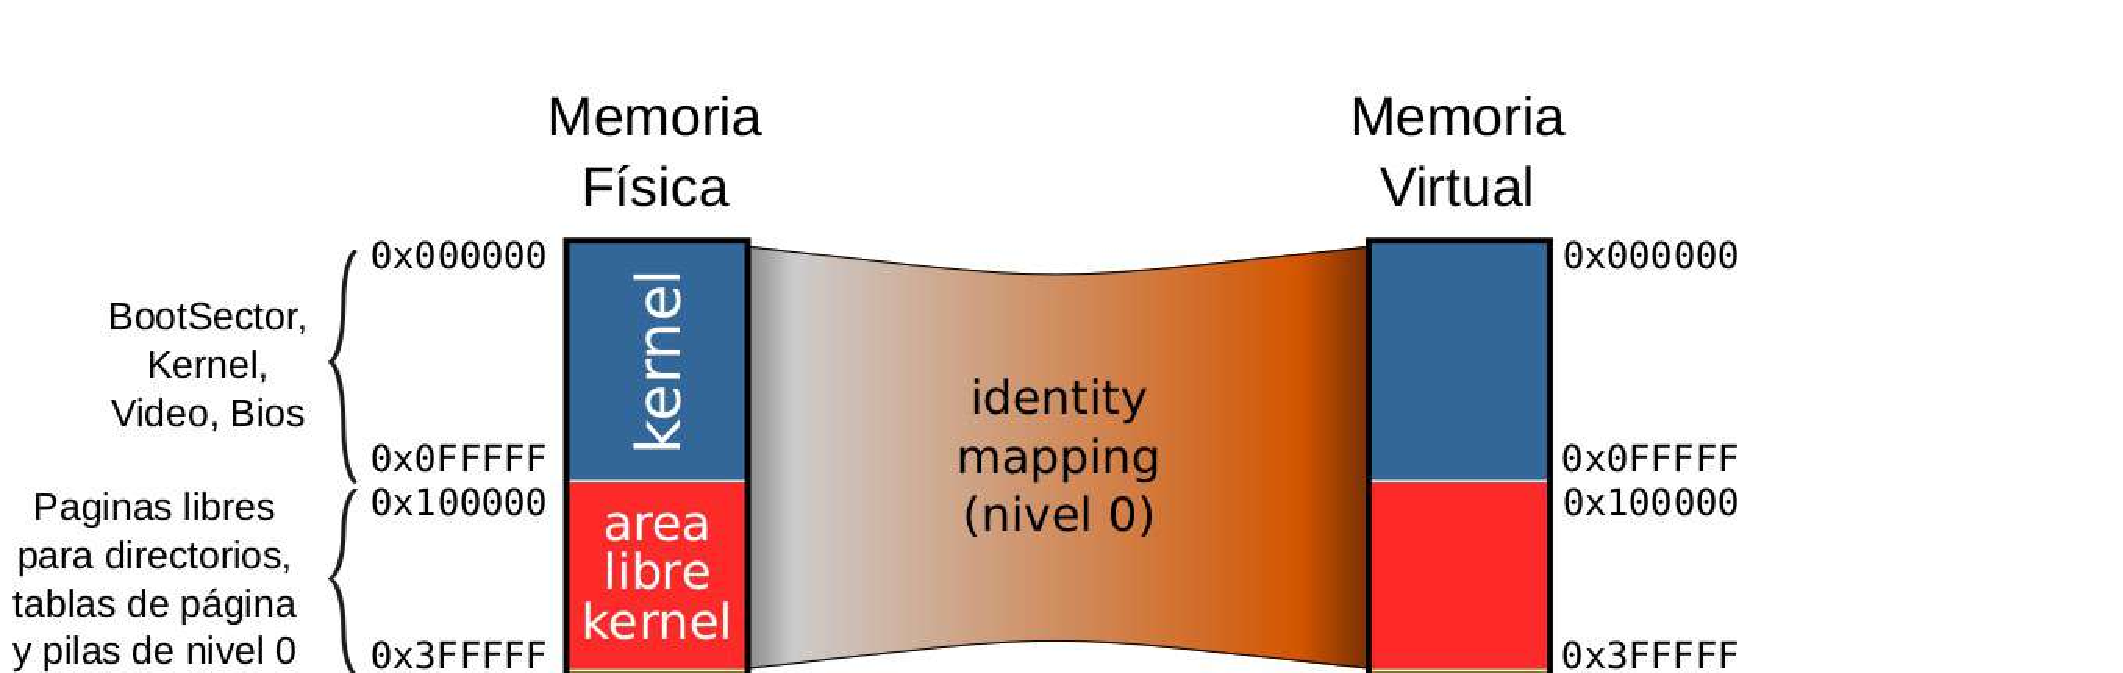
\includegraphics[scale=0.5]{img/MapearKernel.pdf}
	\caption{Mapeo del kernel.}
\end{figure}

\newpage
\subsection{Ejercicio 5}
\justify
Inicialmente y siguiendo lo indicado por el primer item, completamos la función ``mmu_init" \ con la dirección de la primera página libre del kernel (0x100000), y luego completamos la función ``mmu_next_free_kernel_page" \ para que nos devuelva la dirección de la próxima página libre del área libre del kernel.
\justify
Implementamos la función ``mmu_map_page" \ que, dado un cr3, una dirección virtual, una dirección fisica y unos atributos, mapea ambas direcciones. Lo primero que realiza esta función es obtener de la dirección virtual el índice del directorio de tabla de páginas y el índice dentro de la tabla de páginas. También se shiftea cr3 de tal manera de conseguir la dirección de la base del directorio. Luego se fija si la tabla de páginas de esa page_directory_entry está presente y, en caso de que no, la crea pidiendo la próxima página libre del área del kernel y la inicializa con todas las entradas en 0. Una vez creada la tabla de páginas, se completa la entrada correspondiente de la page_directory_entry con la base de la tabla de páginas, los atributos pasados por parámetro(bit de presente, bit de R/W y bit de U/S). Independientemente de si la tabla de página estaba presente o no, se obtiene la base de la página de la dirección física pasada por parámetro y se completa con esto, en la page table entry correspondiente, la base. Posteriormente completamos la misma con los atributos pasados por parámetro.
\justify
Finalmente limpiamos la caché con la funcion tblflush, la cual fue proporcionada por la cátedra.
\justify
Implementamos la función ``mmu_unmap_page" \, la cual recibe como parámetros un cr3 y una dirección virtual, y se encarga de desmapear páginas de memoria. Al igual que la función anterior, a partir de la direccion virtual obtiene el índice del directorio de tabla de páginas y el índice de la tabla de páginas. Del cr3 obtenemos la direccion de la base del directorio de tablas y chequeamos si la page table se encuentra presente en este. En caso de no estar presente devolvemos 0. En el caso contrario, obtenemos la página que nos indica la page table entry y le sumamos el offset de la dirección virtual. Luego completamos esta página con 0s. Limpiamos la caché con tblflush y devolvemos la dirección física a la cual estaba mapeada la dirección virtual.
\justify
Notemos que no chequeamos si la page table entry estaba presente, pero nosotros mantenemos el invariante de que si no está presente toda la page table entry es 0, por ende en este caso, solo devolvería el offset de la dirección virtual.
\justify
Escribimos la rutina ``mmu_init_task_dir" \, la cual se encarga de inicializar el directorio correspondiente para una tarea Rick o Morty. Esta recibe como parámetro la dirección física donde comienza el código de la tarea(code_start), la dirección fisica donde este debe copiarse(phy_start) y la cantidad de páginas de código.
Para esto se crea un directorio de tablas de paǵina pidiendo la pŕoxima página libre de kernel, cuya dirección será el valor del nuevo cr3. Luego, llenamos todas las page directory entry con 0s, y usando la función mmu_map_page realizos el identity mapping del kernel en este nuevo cr3 con los siguientes atributos: P = 1, R/W = 1, y U/S = 0. Tanto en el cr3 actual como en el nuevo, mapeamos 4 páginas a partir de la dirección física phy_start a 4 páginas a partir de la dirección virtual 0x1D000000. Por último, tenemos que copiar el código que se encuentra en la dirección code_start en la dirección virtual 0x1D000000. Notemos que se realiza utilizando el cr3 actual, y por ende, luego de esto tenemos que unmapear las páginas creadas en el mismo. Finalmente, esta función devuelve el nuevo cr3.
 


\subsection{Ejercicio 6}

\justify
Nuevamente modificamos la GDT, esta vez, para agregar las entradas que serán utilizadas como los descriptores de TSS necesarios. En un principio, definimos una entrada para la tarea incial y otra entrada para la tarea Idle cuyos índices en la GDT son 20 y 21 respectivamente. Las bases de estas fueron inicializadas en 0 para luego ser modificadas en tiempo de ejecución. El límite de ambas es 0x67 y está dado por el tamaño de la estructura de la tss definidida por la cátedra. En este caso, la granularidad está seteada en 0 por el tamaño del tss. El bit de AVL está seteado en 0, el bit de P en 1, y el bit de DPL está seteado en 0 ya que el task switch debería poder realizarlo unicamente el kernel. Los bits de tipo están seteados de la siguiente manera: "01001", donde podemos ver que el bit de Busy es 0. Los demás bits están seteados en 0 como indica el manual. Esta configuración va a ser utilizada para el resto de los descriptores de TSS.
%Imagen de los descriptores.
\justify
En el archivo \textbf{tss.h} se encuentra definida una estructura que representa la TSS de una tarea que fue proveída por la cátedra. Luego en \textbf{tss.c} definimos las TSS de la tarea inicial y la tarea Idle. La primera la llenamos con 0s y a la segunda TSS la completamos de la siguiente manera: Como comparte el mismo cr3 con el kernel, cr3 será igual a 0x25000, luego el EIP, como indica el enunciado, será 0x00018000 y EFLAGS será 0x202 (ya que las interrupciones están habilitadas). Tanto los descriptores de datos como el de pila utilizarán el descriptor de datos de nivel 0(RPL = 0) y el selector de código utilizará el descriptor de código de nivel 0(RPL = 0). Por último, el esp y el ebp están seteados en la misma que dirección que la pila del kernel(0x00025000) como lo indica el enunciado. Los demás campos están seteados en 0. Notemos que como utilizamos el cr3 del kernel, todo se encuentra mapeado con identity mapping.
\justify
Para completar la base de los descriptores de TSS, implementamos una función en \textbf{tss.c} llamada define_base_tss, la cual toma como parámetros el indice en la gdt de la tarea y la dirección de la base de la tss. También implementamos dos funciones, tss_init y tss_idle_init, las cuales tienen como objetivo definir la tarea inicial y la tarea idle utilizando la funcion anteriormente mencionada.
\justify
Para ejecutar la tarea idle, en el kernel escribimos el código necesario para completar las tss de la tarea inicial y la tarea idle. En un primer lugar, se cargó en el task register el selector de tss de la tarea inicial. Luego, para efectivamente saltar a la tarea idle, realizamos un jump usando el selector de segmento de la tss de idle(RPL = 0), para así realizar el task switch de la tarea inicial a la tarea idle.
\justify
Por último, en \textbf{tss.c} realizamos una función llamada ``tss_init_task" \ la cual se encarga de completar una TSS con los datos correspondientes a una tarea y completar la base de su descriptor. Esta función toma como parámetro el índice del descriptor del TSS de la tarea en la GDT, la dirección de la base de su TSS, la dirección de una página libre del kernel (la cual sera utilizada para la pila de nivel $0$), el cr3 de la tarea, la dirección virtual donde comienza el código de la tarea y por ultimo la cantidad de paginas de código que posee.
\justify
Lo primero que realiza esta función es llamar a  ``define_base_tt" \ con los parámetros adecuados. Luego definimos la TSS de la siguiente manera: ESP0 es igual a la dirección de la pagina libre del kernel más el tamaño de una página, ya que la pila crece al revés, SS0 se lo carga con un selector del segmento de datos de nivel 0 (RPL=0), CR3 se lo carga con el que fue pasado por parámetro, en EIP se carga la dirección virtual donde comienza el código, eflags se carga con 0x202 (ya que las interrupciones están habilitadas). Ahora debemos cargar los selectores de segmentos de datos y el de pila, estos se cargan utilizando el selector de segmento de datos de nivel 3 (RPL=3) y CS se carga con el selector de segmento de código de nivel 3 (RPL=3). Por último, cargamos ESP Y EBP con la dirección del código sumado a la cantidad de paginas del código multiplicado por el tamaño de una página. Los demás campos se completan con 0.
\subsection{Ejercicio 7}
\justify
Notemos que la maxima cantidad de tareas que puede haber simultáneamente es $24$, las cuales son la inicial, la tarea Idle, Rick, Morty y 10 Mr. Meeseeks por cada uno. Aquellas a las que queremos repartir equitativamente el tiempo son Rick y Morty con sus respectivos Mr. Meeseeks. Teniendo esto en cuenta definimos una estructura llamada scheduler en \textbf{sched.h}, con los siguientes datos:
\begin{itemize}
	\item \textbf{Turno}: es un valor que nos indica si el turno es de Rick o de alguno de sus Mr. Meeseks, o el turno es de Morty o de alguno de sus Mr. Meeseeks. Es $0$ si es turno de una tarea de Rick y $1$ si es de una tarea de Morty.
	\item \textbf{last_task}: es un array de dos valores, el de la primera posición representa la ultima tarea de Rick ejecutada y en la segunda posición la ultima tarea de Morty ejecutada.
	\item \textbf{state}: es un array con 22 valores (la máxima cantidad de tareas simultáneas) que nos indica el estado de cada una de las tareas. Cada tarea puede estar en $3$ estados:
	\begin{itemize}
		\item \textbf{TASK_DEAD}: representa que la tarea está muerta, es decir, el scheduler no debe darle tiempo.
		\item \textbf{TASK_READY}: representa que la tarea está lista para ser ejecutada y por ende esta viva.
		\item \textbf{TASK_EJEC}: representa que la tarea fue la última que se ejecutó o que se está ejecutando. Sin tener en cuenta Idle (este estado no fue necesario).
	\end{itemize} 
	\item \textbf{idx_gdt}: al igual que el anterior es un array de 22 valores, que indica cual es el índice del descriptor de TSS de cada una de las tareas en la GDT. Por ende, podemos obtener un selector de una TSS shifteando hacia la izquierda el índice de la tarea en la GDT.
	\item \textbf{reloj}: otro array de 22 valores, que indica $4$ estados posibles (uno por cada estado del reloj) de cada una de las tareas.   
\end{itemize}
El orden de las tareas en los arrays es el siguiente:
%Poner Imagen
\justify
Ahora debemos inicializar la estructura de datos, para ello creamos un función en \textbf{sched.c} llamada ``sched_init"\ . Lo primero que realiza esta función es inicializar los estados de todas las tareas como TASK_DEAD (las tareas Rick y Morty se inician en TASK_READY en la función ``game_init" \ que luego presentaremos). Luego inicializa los indices de cada una de las tareas en la GDT, teniendo en cuenta que los índices en la GDT respetan el mismo orden que los arrays anteriormente descritos. Por último, inicia las ultimas tareas de Rick y Morty, que en esta caso son las tareas principales, e inicia turno con $1$ para que el próximo turno corresponda a Rick.

\justify
Siguiendo lo indicado en el item b creamos un función ``sched_next_task"\ encargada de devolver el selector de segmento de TSS de la siguiente tarea a ejecutar. Si el juego terminó, es decir alguna tarea principal fue desalojada o si capturaron todas las megasemillas (esto lo vamos a explicar mejor en el ejercicio $8$), devolvemos el selector de la tarea Idle. En caso contrario, el juego no terminó por ende actualizamos el estado de la última tarea que ejecuto (si sigue viva). Luego, cambiamos el turno y buscamos la próxima tarea a ejecutar que pertenezca al turno actual. Para esto, realizamos una búsqueda lineal y si nos pasamos de rango volvemos al principio. Una vez encontrada la próxima tarea a ejecutar actualizamos last_task del turno actual. Si la siguiente tarea a ejecutar es un Mr. Meeseeks, actualizamos la maxima cantidad de casillas que se puede mover (se explicara más en el ejercicio $8$). Por último, actualizamos el estado de la proxima tarea a ejecutar, cambiamos el estado del reloj de la misma y devolvemos el selector de su TSS (RPL=0).
\justify
Para realizar el cambio de tarea, modificamos la rutina de atención del reloj (ISR 32). Definimos una variable en isr.asm llamada sched_task_selector, la cual se utiliza para guardar el selector de TSS de la tarea a la que queremos saltar y poder realizar un jmp far. Llamamos a la función ``sched_next_task"\ la cual nos devuelve en ax el resultado. Comparamos el resultado con el almacenado en el Task Register. En caso de que sean iguales, no hacemos nada. Caso contrario, guardamos en sched_task_selector el nuevo selector de TSS y realizamos un jmp far. Como se pintan los relojes lo vamos a tratar mas adelante en el ejericio $9$.
\justify
Análogamente modificamos las rutinas de interrupciones de software para que salten a la tarea Idle cuando son invocadas.

\justify
Para atender a la excepciones creamos una función llamada ``sched_desalojar"\ en \textbf{sched.c}. La misma realiza una busqueda lineal para obtener la tarea que se está ejecutando (se puede utilizar last_task y turno para realizar esto). Se actualiza el estado de la misma y realizamos dos cosas distintas dependiendo si es una tarea principal o no (se verá mas en detalle en el ejercicio $8$). Por último, llamamos a una función llamada saltar_idle() definida en isr.asm.


\justify
Para implementar el debugger utilizamos la variable debug_state, esta puede tomar $3$ valores los cuales nos indicaran si modo debugger esta apagado (0), modo debugger esta activado (1) o si se esta printeando en pantalla el debugger (2).

\justify
Creamos dos funciones ``copiar_pantalla"\ y ``devolver_pantalla"\ en \textbf{screen.c} y una matriz de píxeles de 50x80 llamada copia_de_pantalla. Al llamar a ``copiar_pantalla"\ se copian los píxeles actuales de la pantalla en copia_de_pantalla y al llamar a ``devolver_pantalla"\ se pinta la pantalla con los píxeles indicados por copia_de_pantalla.
\justify
Se modifico la rutina de atención de las excepciones para que pushee todos los registros de propósito generales con pushad, luego pushee los selectores de datos y por ultimo el numero de excepción que ocurrió. Luego de esto se llama a copiar pantalla, se chequea si el estado de debug_state es $1$ y en caso de que lo sea se llama a ``imprimir_debug"\ que se encuentra definido en \textbf{screen.c}. Por ultimo, independientemente del valor de debug_state se desaloja la tarea actual llamando a ``sched_desalojar"\, la cual se encargara de saltar a la tarea Idle. Notemos que no restauramos la pila, ya que la tarea actual nunca mas será atendida por el scheduler, a menos que se la vuelva a crear si es una tarea Mr Meeseeks, pero en este caso será una tarea limpia.

\justify
La función ``imprimir_debug"\ toma como parámetros los registros de propósito general y los selectores de datos al momento de atender la excepción. Notemos que todos estos registros poseen el mismo valor que tenían antes de producirse la excepción, menos el registro ESP el cual será el de nivel 0. Como se produjo un cambio en el nivel de privilegio, el estado de la pila antes de pushear cualquier registro en la rutina de atención de excepciones es el siguiente:
%Poner Imagen
Cuando hacemos un pushad el valor de ESP que se pushea es el de antes de realizar esta operación. Por ende, los elementos que se ven en la imagen están en las posiciones siguientes al ESP pusheado. Por lo cual, podemos obtener estos valores leyendo [ESP], [ESP+4], $\dots$, pero notemos que tenemos que diferenciar si la excepción tiene código de error o no. Teniendo esto en cuenta podemos obtener los valores de la pila de nivel 0. Ahora, nos falta saber los valores de los cr's, pero para esto tenemos la funciones proveidas por la cátedra ``rcr0"\, ``rcr2"\, ``rcr2"\ y ``rcr3"\ .

\justify
Por último debemos imprimir los valores del stack y del backtrace. Para los valores del stack utilizamos el esp de la pila de nivel $3$ de la tarea e imprimimos los $3$ primeros valores ,teniendo en cuenta de estar en el rango de la tarea. Para el backtrace, usamos el $ebp$, asumiendo que se respeta la convención C. Con el mismo, podemos obtener con [ebp+4] la dirección de retorno de la función y con [ebp] el antiguo valor de ebp. Realizamos este proceso iterativamente 3 veces, colocando 0's si ebp o ebp+4 no estan en el rango de la tarea. Para saber si esta en el rango, utilizamos los arrays min_esp_task y max_esp_task, declarados en \textbf{game.h}, que nos indican el rango de memoria de cada tarea. Esto se puede realizar de esta manera ya que estamos utilizando segmentación flat.

%Poner imagen de como queda la pila despues del armado de stackframe

\justify
Modificamos la rutina de interrupción del teclado para que si el scan code detecta que se presiona la tecla ``Y"\ se llame a la función ``change_state_debug"\ que se encuentra definida en \textbf{sched.c} la cual cambia los estados de debug_state como indica el enunciado y si esta mostrando en pantalla el debugger se utiliza la función ``devolver_pantalla"\ . La rutina de reloj también fue modificada para que no realice nada si debug_state es igual a $2$.


\subsection{Ejercicio 8}
\justify
Notemos que Rick y Morty pueden poseer a lo sumo 10 Mr Meeseeks simultáneamente. Las direcciones virtuales donde debe estar el código y la pila de los Mr Meeseeks es a partir de 0x08000000. Podemos entonces definir que los espacios para cada tarea Mr Meeseeks que se pueda crear sea fijo, quedando así para cada tarea principal la siguiente asignación de espacios en su CR3:
%Imagen en que rangos virtuales van a estar cada Mr M

\justify
Definimos las siguientes estructuras en \textbf{juego.h}:
\begin{itemize}
	\item \textbf{posicion}: posee dos valores x, y que representan una posición en el mapa.
	\item \textbf{juego}: posee los siguientes datos:
	\begin{itemize}
		\item \textbf{posiciones_Mr_M}: una array de posiciones de tamaño 20 (igual a la cantidad maxima de tareas Mr Meeseeks), que indica en que posición esta cada tarea Mr Meeseeks, si es que se encuentra viva.
		\item \textbf{posicion_megasemillas}: un array de tamaño 40 (igual a la cantidad de megasemillas iniciales), que indica en que posición se encuentran las megasemillas. Si la semilla no se encuentra mas en el mapa se guarda el valor -1 en x e y (como son unsigend int este valor es 0xFFFFFFFF).
		\item \textbf{cant_Megasemillas}: contiene la cantidad de megasemillas que se encuentran en el mapa actualmente.
		\item \textbf{puntajes}: es un array de dos valores. El primero indica el puntaje de Rick y el segundo el de Morty.
		\item \textbf{page_stack0_Mr_M}: es un array de tamaño 20 que contiene las direcciones de las paginas para la pila de nivel 0 de cada tarea. Se podría usar una nueva pagina para cada nueva tarea que se crea, pero esto seria ineficiente ya que podemos reutilizarlas.
		\item \textbf{color_players}: es un array de dos valores. El primer valor representa el color de Rick, y el segundo el color de Morty.
		\item \textbf{max_move_Mr_M}: es un array de tamaño 20 que  indica el máximo movimiento que puede realizar cada tarea Mr Meeseeks con la syscall Move. Este valor no se guarda explícitamente, sino que cuando se crea un Mr Meeseeks en este array se guarda el valor 16. Luego, cada vez que el scheduler indique que la próxima tarea a ejecutar es un Mr Meeseeks se reduce el valor de esta tarea en el array en 1, a menos que sea igual a 2. Entonces el máximo movimiento que puede realizar un Mr Meeseeks es en realidad este valor divido $2$.
		\item \textbf{uso_portal_gun}: es un array de 20 posiciones que indica si una tarea Mr Meeseeks ya uso la syscall use_portal_gun.
		\item \textbf{cr3_players}: es un array de dos posiciones. En la primera contiene el CR3 de la tarea Rick, y en la segunda posición el CR3 de la tarea Morty.
	\end{itemize}
\end{itemize}
Los arrays que contiene datos sobre los Mr Meeseeks tendrán el siguiente orden de tareas:
%figura 
\justify
De esta forma dado el índice de una tarea Mr Meeseeks en el scheduler, se puede obtener el índice en estos arrays restando $2$ y se puede obtener qué número de Mr Meeseeks es para cada tarea principal restando $2$ y luego dividiendo por $2$.
\justify
Para la distribucion de semillas en la pantalla del juego, en primera instancia se completa el array de posicion_megasemillas, nombrado anteriormente, con posiciones aleatorias dentro del mapa. Una vez hecho esto, la funcion ''actualizar_pantalla" se encarga de recorrer este array y mostrar en pantalla todas las semillas que tienen una posición válida.
\justify
Desarrollamos la lógica de la rutina meeseeks con ayuda de una función en C llamada "servicio_meeseeks". Dicha función recibe como parámetro la dirección virtual del código de un meeseek, y las coordenadas x e y donde el meeseek debe ubicarse en el mapa. En primer lugar, en esta función chequeamos que el código del meeseek se encuentre en el rango de direcciones específico de las tareas y que la posicion pasada por parámetro sea una posicion váĺida en el mapa. En caso de no cumplir estos requisitos, se desalojará a la tarea que llamó al servicio. Posteriormente, buscamos en el array de state, el índice de tarea que le correspondería a este nuevo meeseek creado. En caso de no haber lugares disponibles el meeseek no se crea. Luego, verificamos si en la posición donde se va a crear el meeseek hay una semilla. En caso de haberla, se aumenta el puntaje del jugador que llamó al servicio,y se actualiza la información de esa semilla. Si no se cumple ninguna de las condiciones anteriores, procedemos a realizar el proceso para ubicar al meeseek en el mapa. Primero, actualizamos la información necesaria de esta nueva tarea en los distintos array mencionados anteriormente. Luego, mapeamos las dos páginas del meeseek creado, ubicadas de acuerdo a su índice de tarea, en las dos páginas de la posición del mapa que corresponde. Una vez mapeadas, copiamos el código de la tarea, ubicado a partir de la direccion pasada por parámetro, en la dirección que le corresponde según su índice de tarea. Por último, iniciamos la tss de esta tarea recien creada con la función ``tss_init_task" \ y actualizamos el estado de la tarea en el scheduler. Esta función retorna la dirección virtual que le corresponde a esta tarea a partir de 0x80000000. 





\end{document}

